\subsection{Caso 3: la misión simulada}
\label{sec:resultados}

Cada misión libera a los insectos por un boquete de un colapso sintético con unos \areaLibre~m$^2$ de huecos; la
persona está inmóvil, a un recorrido medio de \distVictima~m. Cada configuración se corrió \numCorridas{} veces en
\numMapas{} colapsos: \numMisiones{} misiones de una hora, con un margen de unos $\pm5$ puntos (95~\%).

\textbf{Validación.} En una arena de $1\times1$~m el insecto simulado camina \valAndaNat{} del tiempo sin estímulos
(publicado: $0.37\pm0.20$), hace pausas de \valPausaNat~s ($36.8\pm24.1$) y suelta la pared con probabilidad
\valSalidaNat{} (0.005); con comandos, \valAndaCom{} (0.643) y \valSalidaCom{}
(0.052)~\cite{dirafzoon2017,tranngoc2024}. Solo difiere la pausa con comandos: \valPausaCom~s frente a 5.6~s, de modo
que el modelo es conservador (tabla~\ref{tab:validacion}).

\begin{table}[!htb]
\centering\footnotesize
\caption{Marcha simulada frente a la publicada.}
\label{tab:validacion}
\rowcolors{2}{SoftGray}{white}
\begin{tabularx}{0.86\textwidth}{@{}>{\raggedright\arraybackslash}X r r@{}}
\toprule
\rowcolor{TableHead} \textbf{Medida} & \textbf{Publicado} & \textbf{Simulación} \\
\midrule
Fracción del tiempo caminando, sin estímulos & $0.37\pm0.20$ & \valAndaNat \\
Pausa media, sin estímulos (s) & $36.8\pm24.1$ & \valPausaNat \\
Probabilidad de soltar la pared, sin estímulos & 0.005 & \valSalidaNat \\
Fracción del tiempo caminando, con comandos & 0.643 & \valAndaCom \\
Probabilidad de soltar la pared, con comandos & 0.052 & \valSalidaCom \\
Pausa media, con comandos (s) & 5.55 & \valPausaCom \\
\bottomrule
\end{tabularx}
\end{table}

\textbf{Cuatro políticas.} La \textbf{pasiva} solo detecta; la \textbf{antipausa} da un pulso de avance cuando el
insecto lleva 15~s quieto; la \textbf{estocástica} añade giros al azar, y la \textbf{guiada}, la del núcleo, gira
además hacia el calor (figura~\ref{fig:politicas} y tabla~\ref{tab:politicas}); la figura~\ref{fig:mapa} muestra una
misión.

\begin{figure}[!htb]
\centering
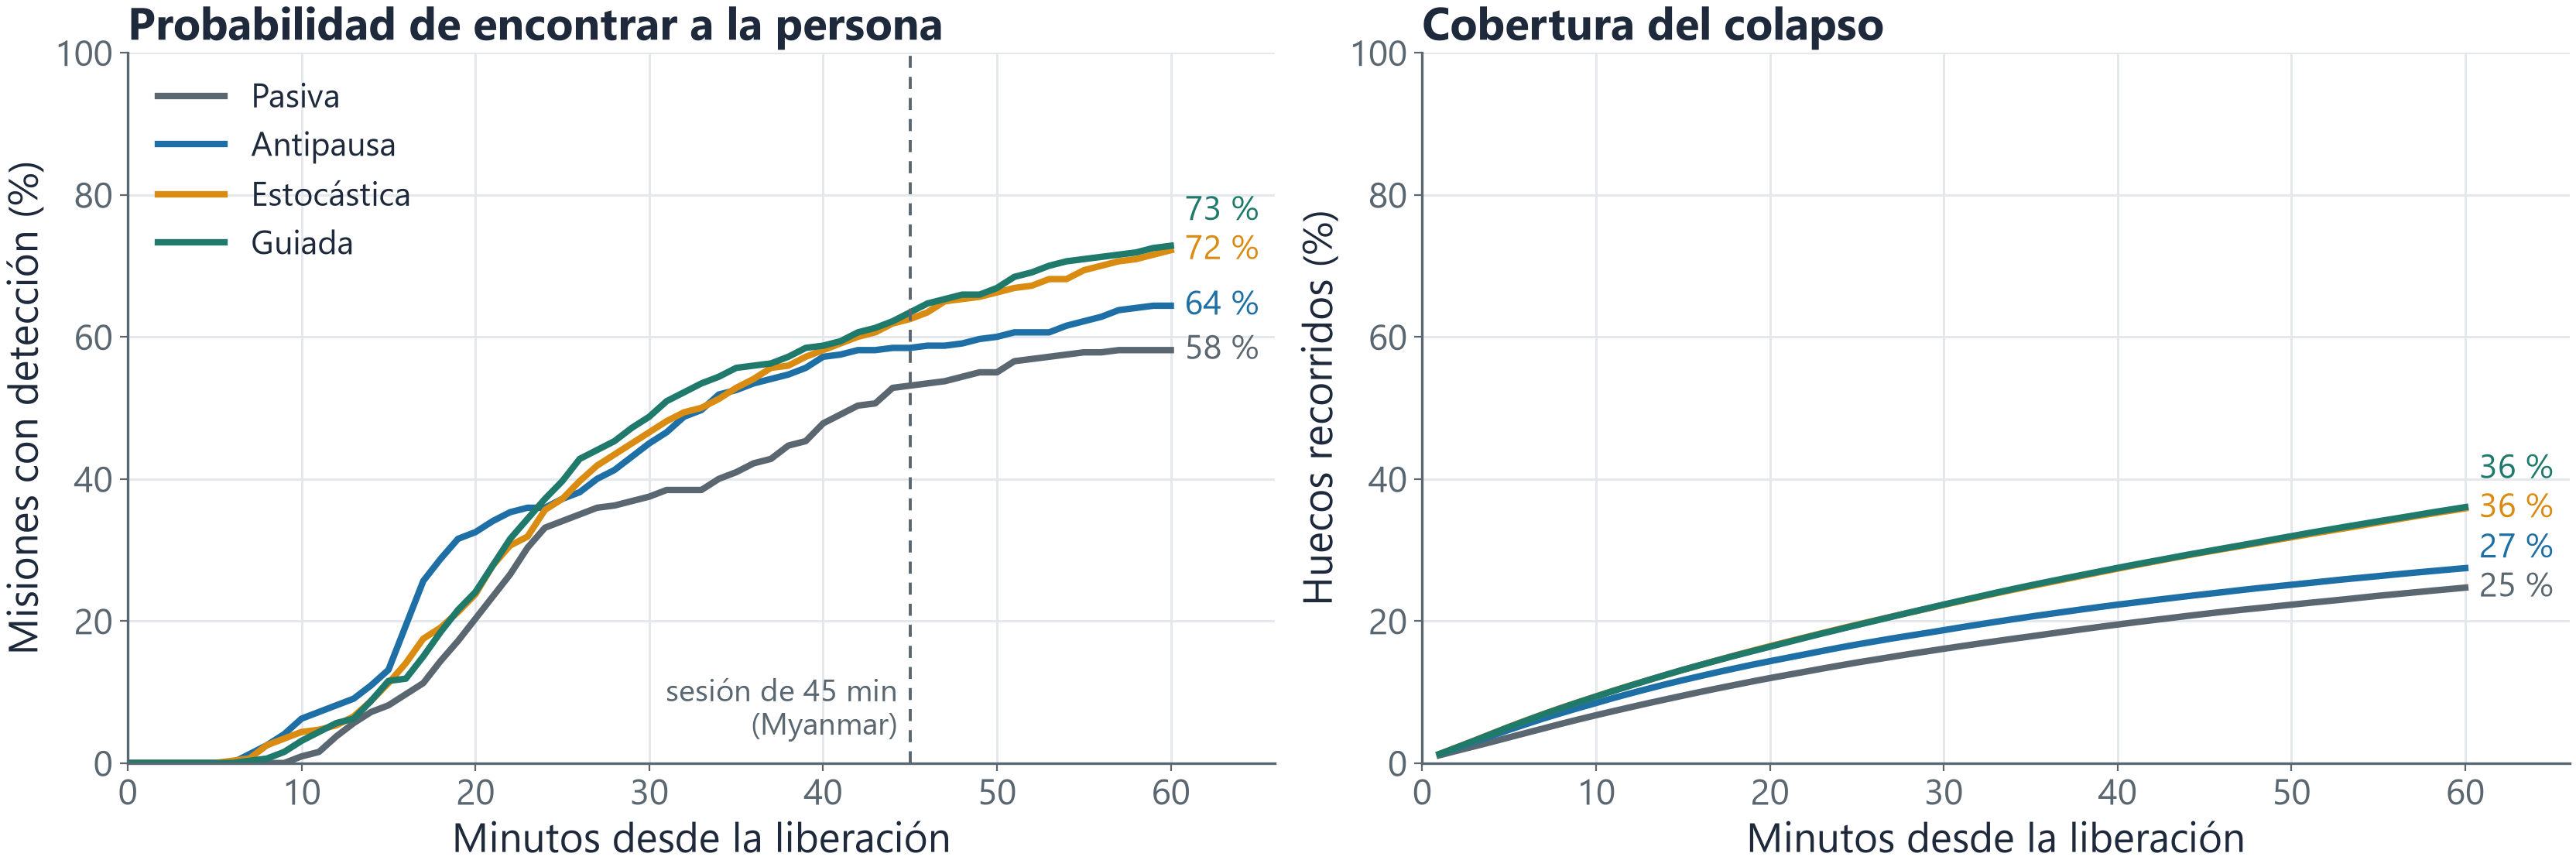
\includegraphics[width=0.98\textwidth]{figs/resultados_politicas.png}
\caption{Diez insectos, \numMisiones{} misiones por política. Izquierda: misiones en que algún insecto confirma a la
persona. Derecha: fracción de los huecos por los que pasó al menos un insecto.}
\label{fig:politicas}
\end{figure}

\begin{table}[!htb]
\centering\footnotesize
\caption{Resultados por política con diez insectos.}
\label{tab:politicas}
\rowcolors{2}{SoftGray}{white}
\begin{tabularx}{\textwidth}{@{}>{\bfseries\raggedright\arraybackslash}X r r r r r r r r@{}}
\toprule
\rowcolor{TableHead} & \multicolumn{4}{c}{\textbf{Detección acumulada (\%)}} & \textbf{Mediana} & \textbf{Cobertura} & \textbf{Estímulos por} & \textbf{Tiempo} \\
\rowcolor{TableHead} \textbf{Política} & 15 min & 30 min & 45 min & 60 min & (min) & (\%) & insecto y hora & caminando (\%) \\
\midrule
\tablaPoliticas
\bottomrule
\end{tabularx}
\end{table}

La ganancia viene de mantener al insecto en movimiento y despegarlo de las paredes; girar hacia el calor casi no
añade, porque solo actúa dentro del alcance de la matriz. En el primer cuarto de hora las políticas no se
distinguen, y el costo es bajo: unos \estGuiada{} estímulos por insecto y por hora.

\begin{figure}[!htb]
\centering
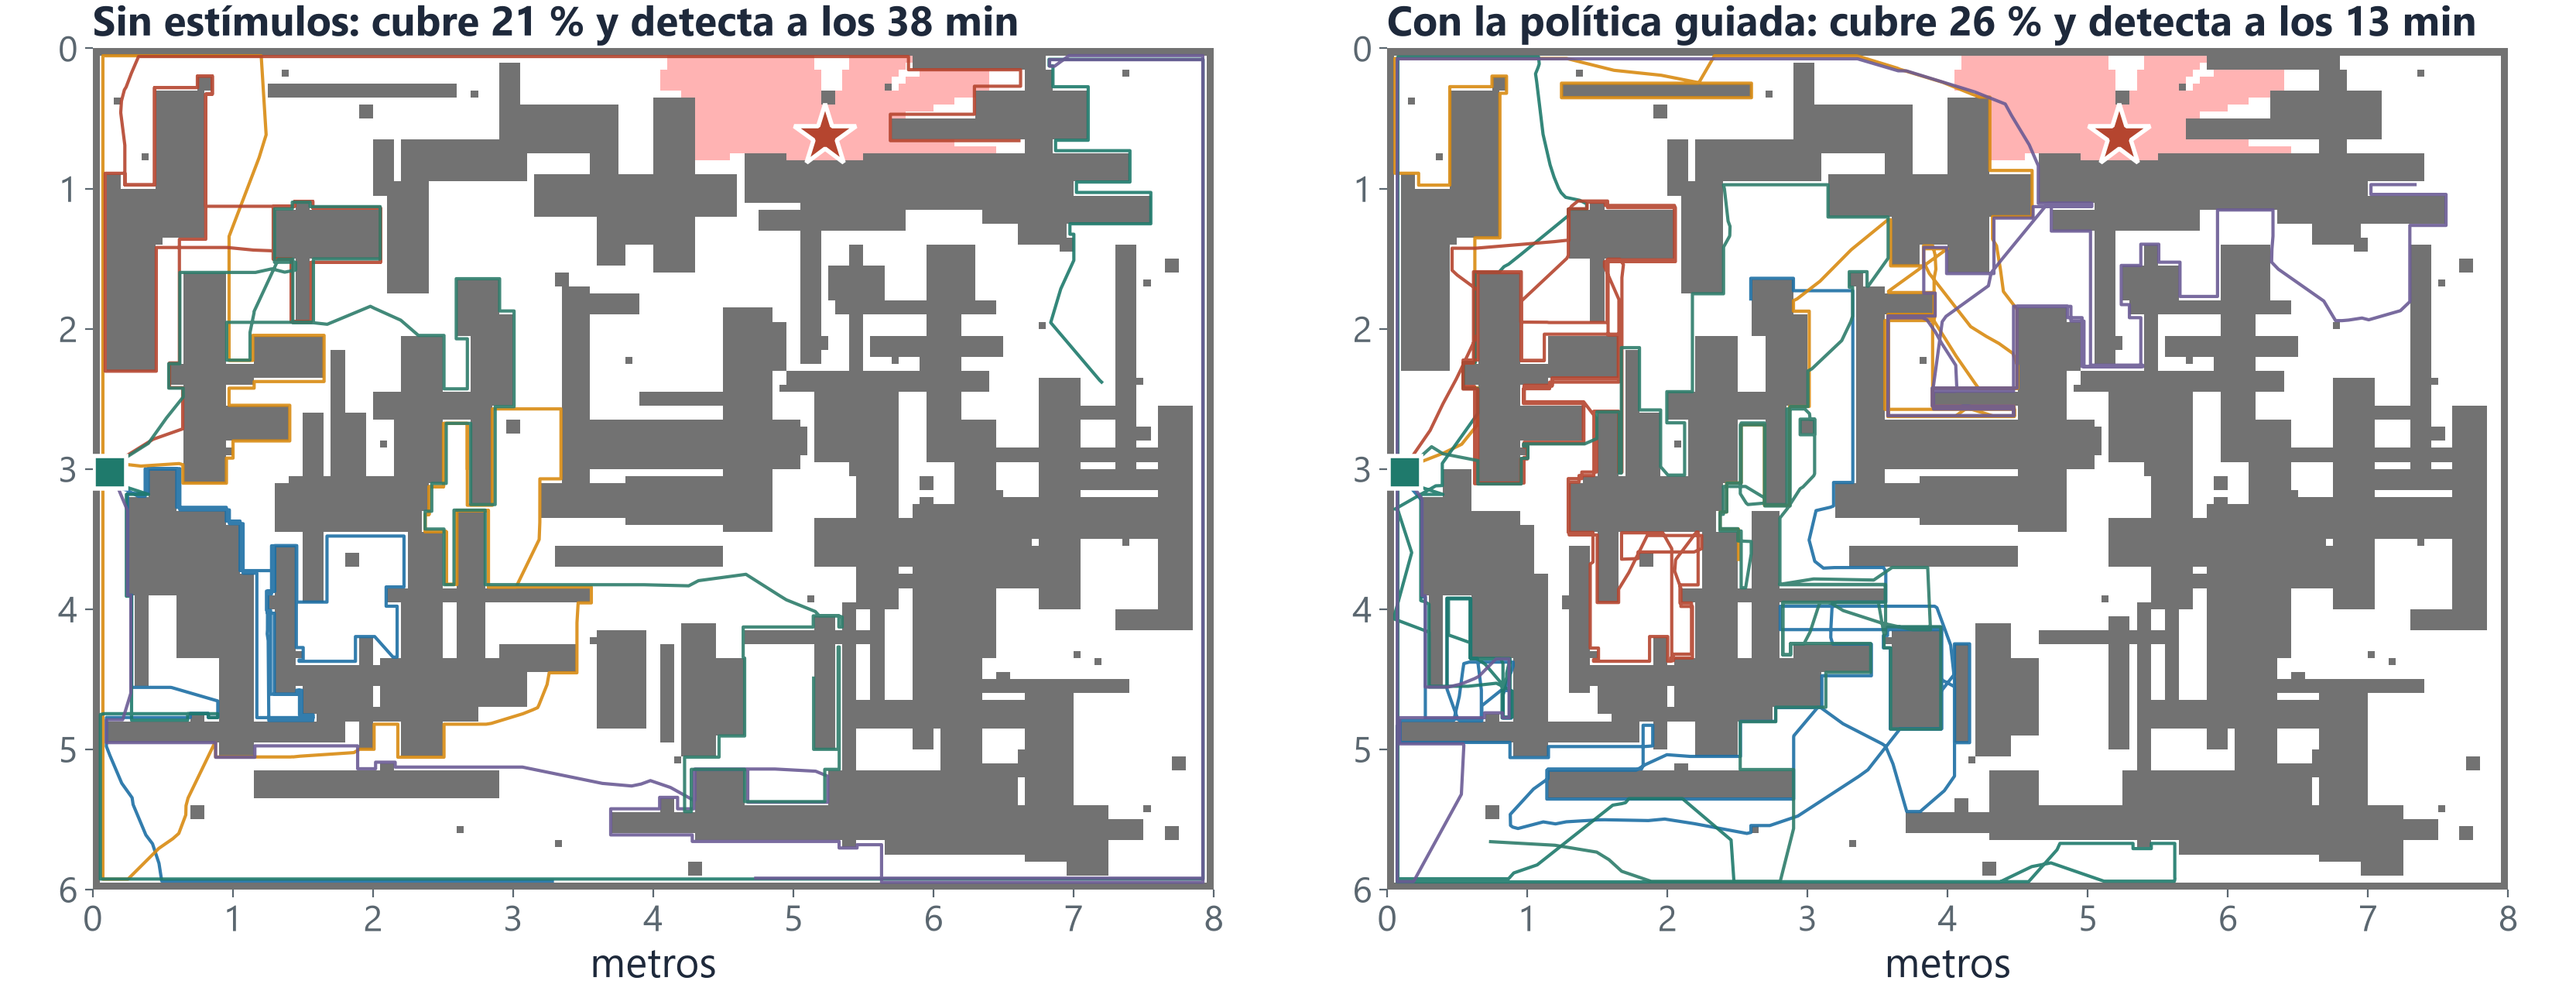
\includegraphics[width=0.92\textwidth]{figs/mapa_trayectorias.png}
\caption{Una misión de ejemplo: seis insectos durante 45~min en el mismo colapso. Cuadro verde: entrada; estrella:
persona; zona sombreada: desde donde la matriz confirma.}
\label{fig:mapa}
\end{figure}

\textbf{El colapso pesa más que la política} (figura~\ref{fig:mapaenjambre}a). Según el colapso, la detección en una
hora va de \mapaMinPasiva{} a \mapaMaxPasiva~\% sin estímulos y de \mapaMinGuiada{} a \mapaMaxGuiada~\% con la
guiada, que gana en \mapasGanaGuiada{} de los \numMapas{}, empata en \mapasEmpate{} y pierde en
\mapasPierdeGuiada. En el mejor caso pasa de \mapaMejorPasiva{} a \mapaMejorGuiada~\%; en el peor, de
\mapaPeorPasiva{} a \mapaPeorGuiada~\%, porque ahí seguir la pared lleva directo a la persona. Un enjambre mixto, con
cinco de cada uno, conserva el promedio (\mixtoSesenta~\%) y quita el caso malo (\mixtoPeor~\% en lugar de
\mapaPeorGuiada~\%): es la configuración que se recomienda.

\textbf{Tamaño del enjambre} (figura~\ref{fig:mapaenjambre}b). Uno solo encuentra a la persona en una de cada cuatro
misiones (\enjHoraPasivaUno{} y \enjHoraGuiadaUno~\%). Con veinte, la guía sube la detección de
\enjHoraPasivaVeinte{} a \enjHoraGuiadaVeinte~\%. Diez guiados (\enjHoraGuiadaDiez~\%) rinden como entre veinte y
cuarenta sin guiar: la política equivale a duplicar o triplicar el enjambre.

\begin{figure}[!htb]
\centering
\begin{subfigure}{0.50\textwidth}
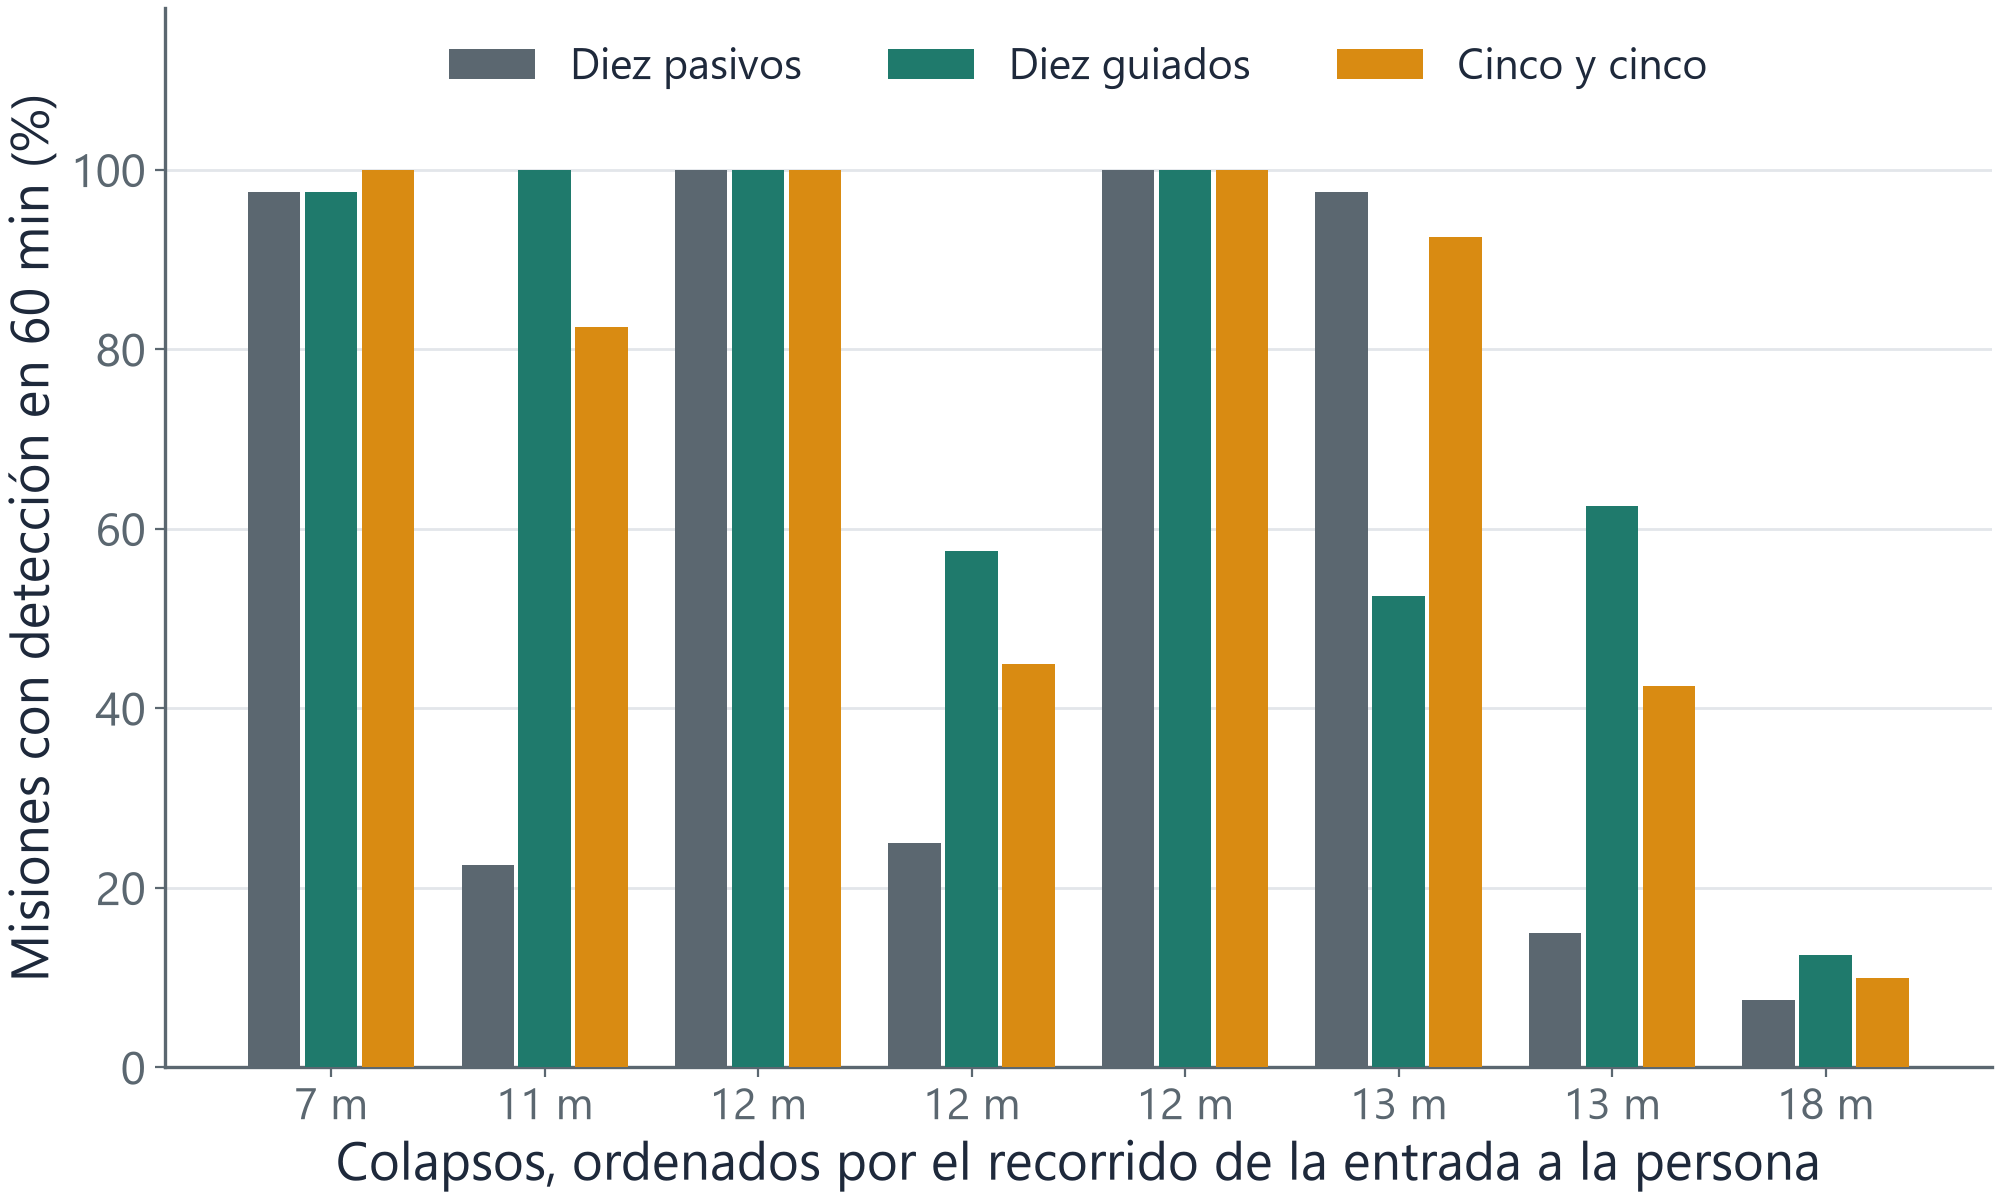
\includegraphics[width=\linewidth]{figs/por_mapa.png}
\caption{Detección a 60~min en cada colapso.}
\end{subfigure}\hfill
\begin{subfigure}{0.46\textwidth}
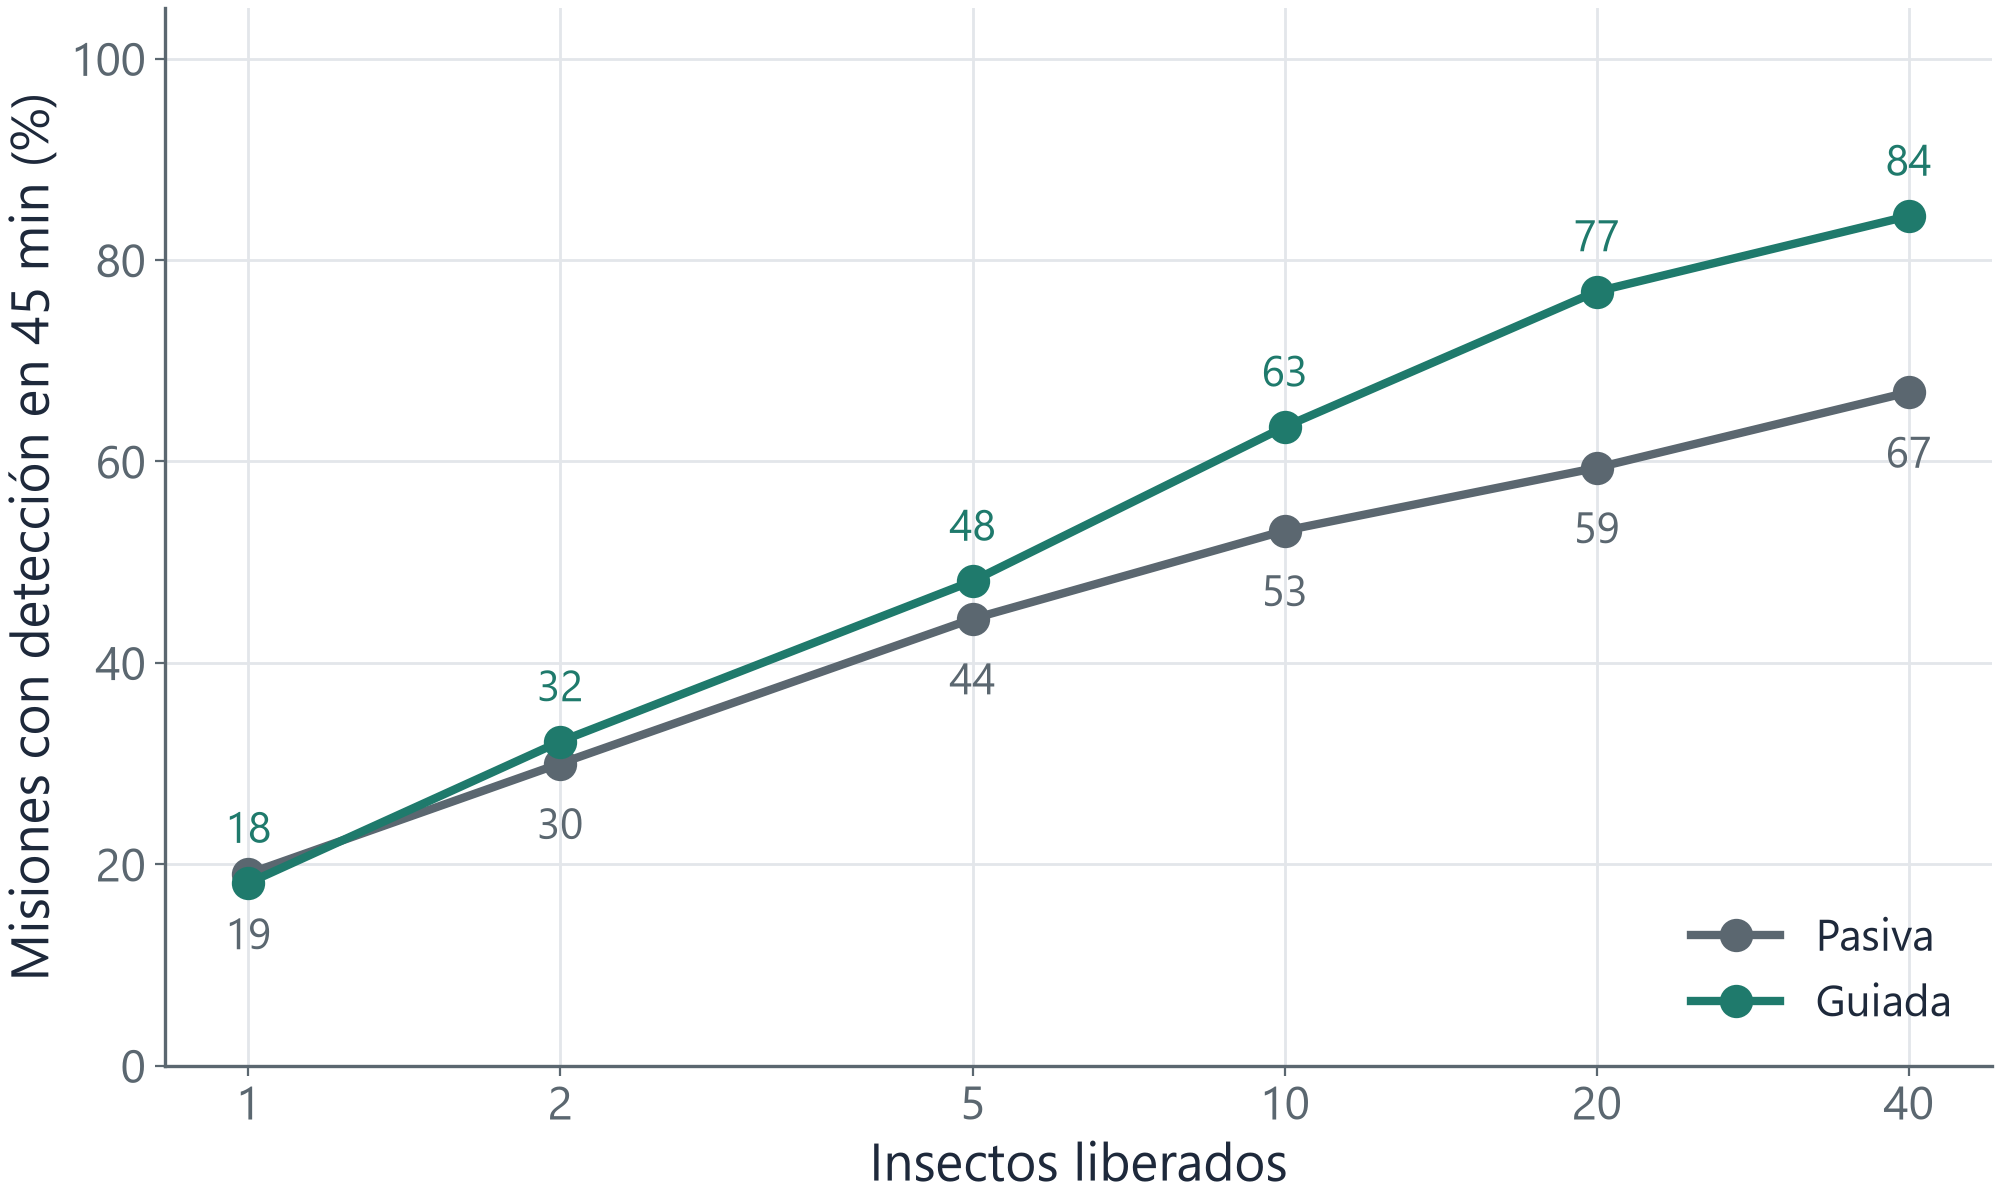
\includegraphics[width=\linewidth]{figs/enjambre.png}
\caption{Detección a 45~min según el número de insectos.}
\end{subfigure}
\caption{Efecto de la geometría del colapso y del tamaño del enjambre.}
\label{fig:mapaenjambre}
\end{figure}

\textbf{Sensor y habituación.} Con la guiada, la matriz de $8\times8$ detecta en una hora en \senOchoSesenta~\% de las
misiones y la de $32\times32$ en \senTreintaDosSesenta~\%: la que se consigue en México pierde pocos puntos. En
misiones de dos horas con pulsos unipolares, estimular sin límite aplica \habEstSinLimite{} estímulos por insecto y
por hora y deja la respuesta en \habRespSinLimite~\%; con el presupuesto son \habEstDosificado{} y
\habRespDosificado~\%, con una detección prácticamente igual (\habDetSinLimite{} y \habDetDosificado~\%). El
argumento para dosificar es el animal, no el rendimiento (figura~\ref{fig:sensorhab}).

\begin{figure}[!htb]
\centering
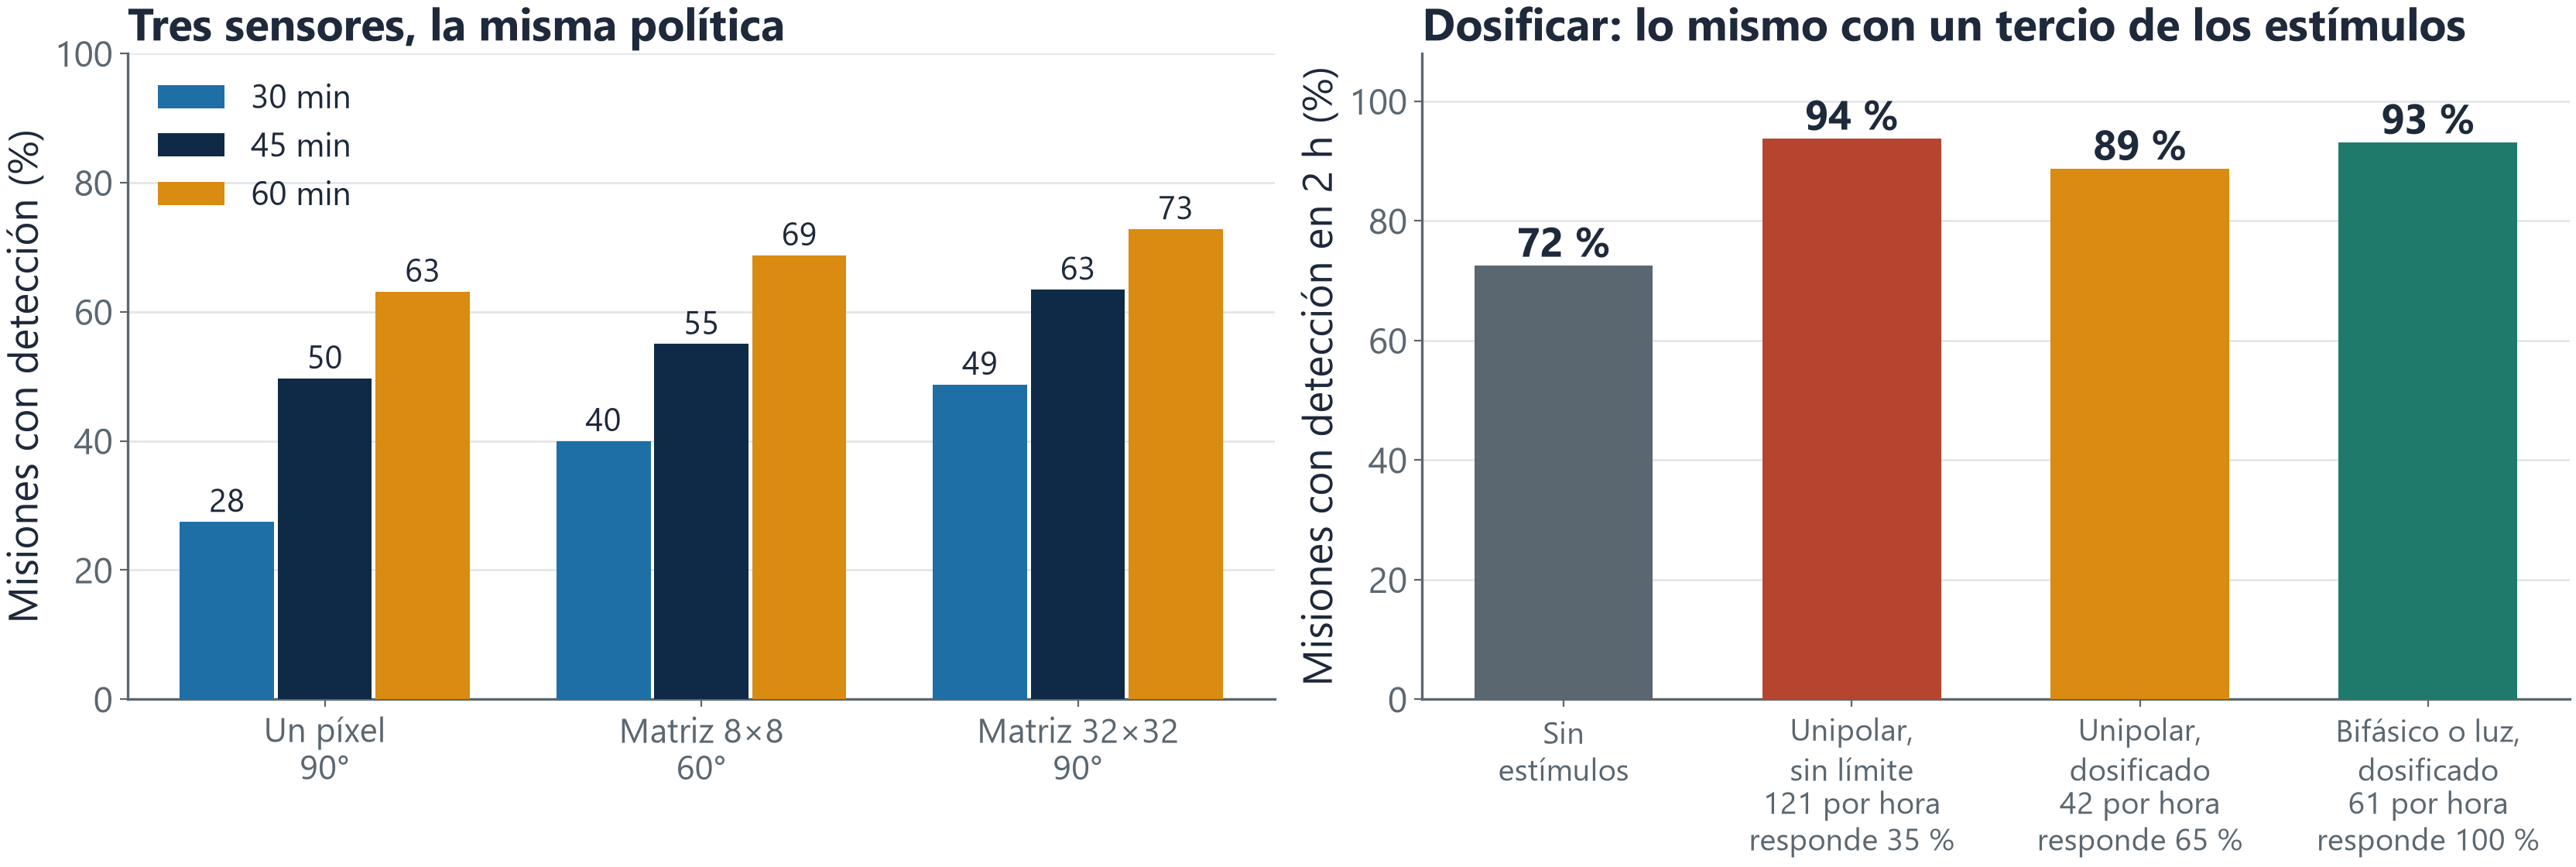
\includegraphics[width=0.94\textwidth]{figs/sensores_habituacion.png}
\caption{Izquierda: política guiada con tres sensores. Derecha: misiones de dos horas con pulsos unipolares, con y
sin dosificación, frente a un estímulo que no habitúa.}
\label{fig:sensorhab}
\end{figure}

\textbf{Sensibilidad} (figura~\ref{fig:sensibilidad}). Doce supuestos se movieron uno a la vez en cuatro colapsos.
Cuatro cambian el resultado más que el margen de muestreo: el largo del tramo recto (de \sensTramoBajoGuiada{} a
\sensTramoAltoGuiada~\%), la velocidad que quita la carga (de \sensCargaBajoGuiada{} a \sensCargaAltoGuiada~\% si
resta 30~\%), la duración de las pausas (de \sensPausaBajoGuiada{} a \sensPausaAltoGuiada~\%) y la velocidad de
marcha (de \sensVelocidadBajoGuiada{} a \sensVelocidadAltoGuiada~\%). La política tolera la incertidumbre sobre el
estímulo, que es lo peor conocido; lo que más importa es cuánto y qué tan rápido camina el insecto.

\begin{figure}[!htb]
\centering
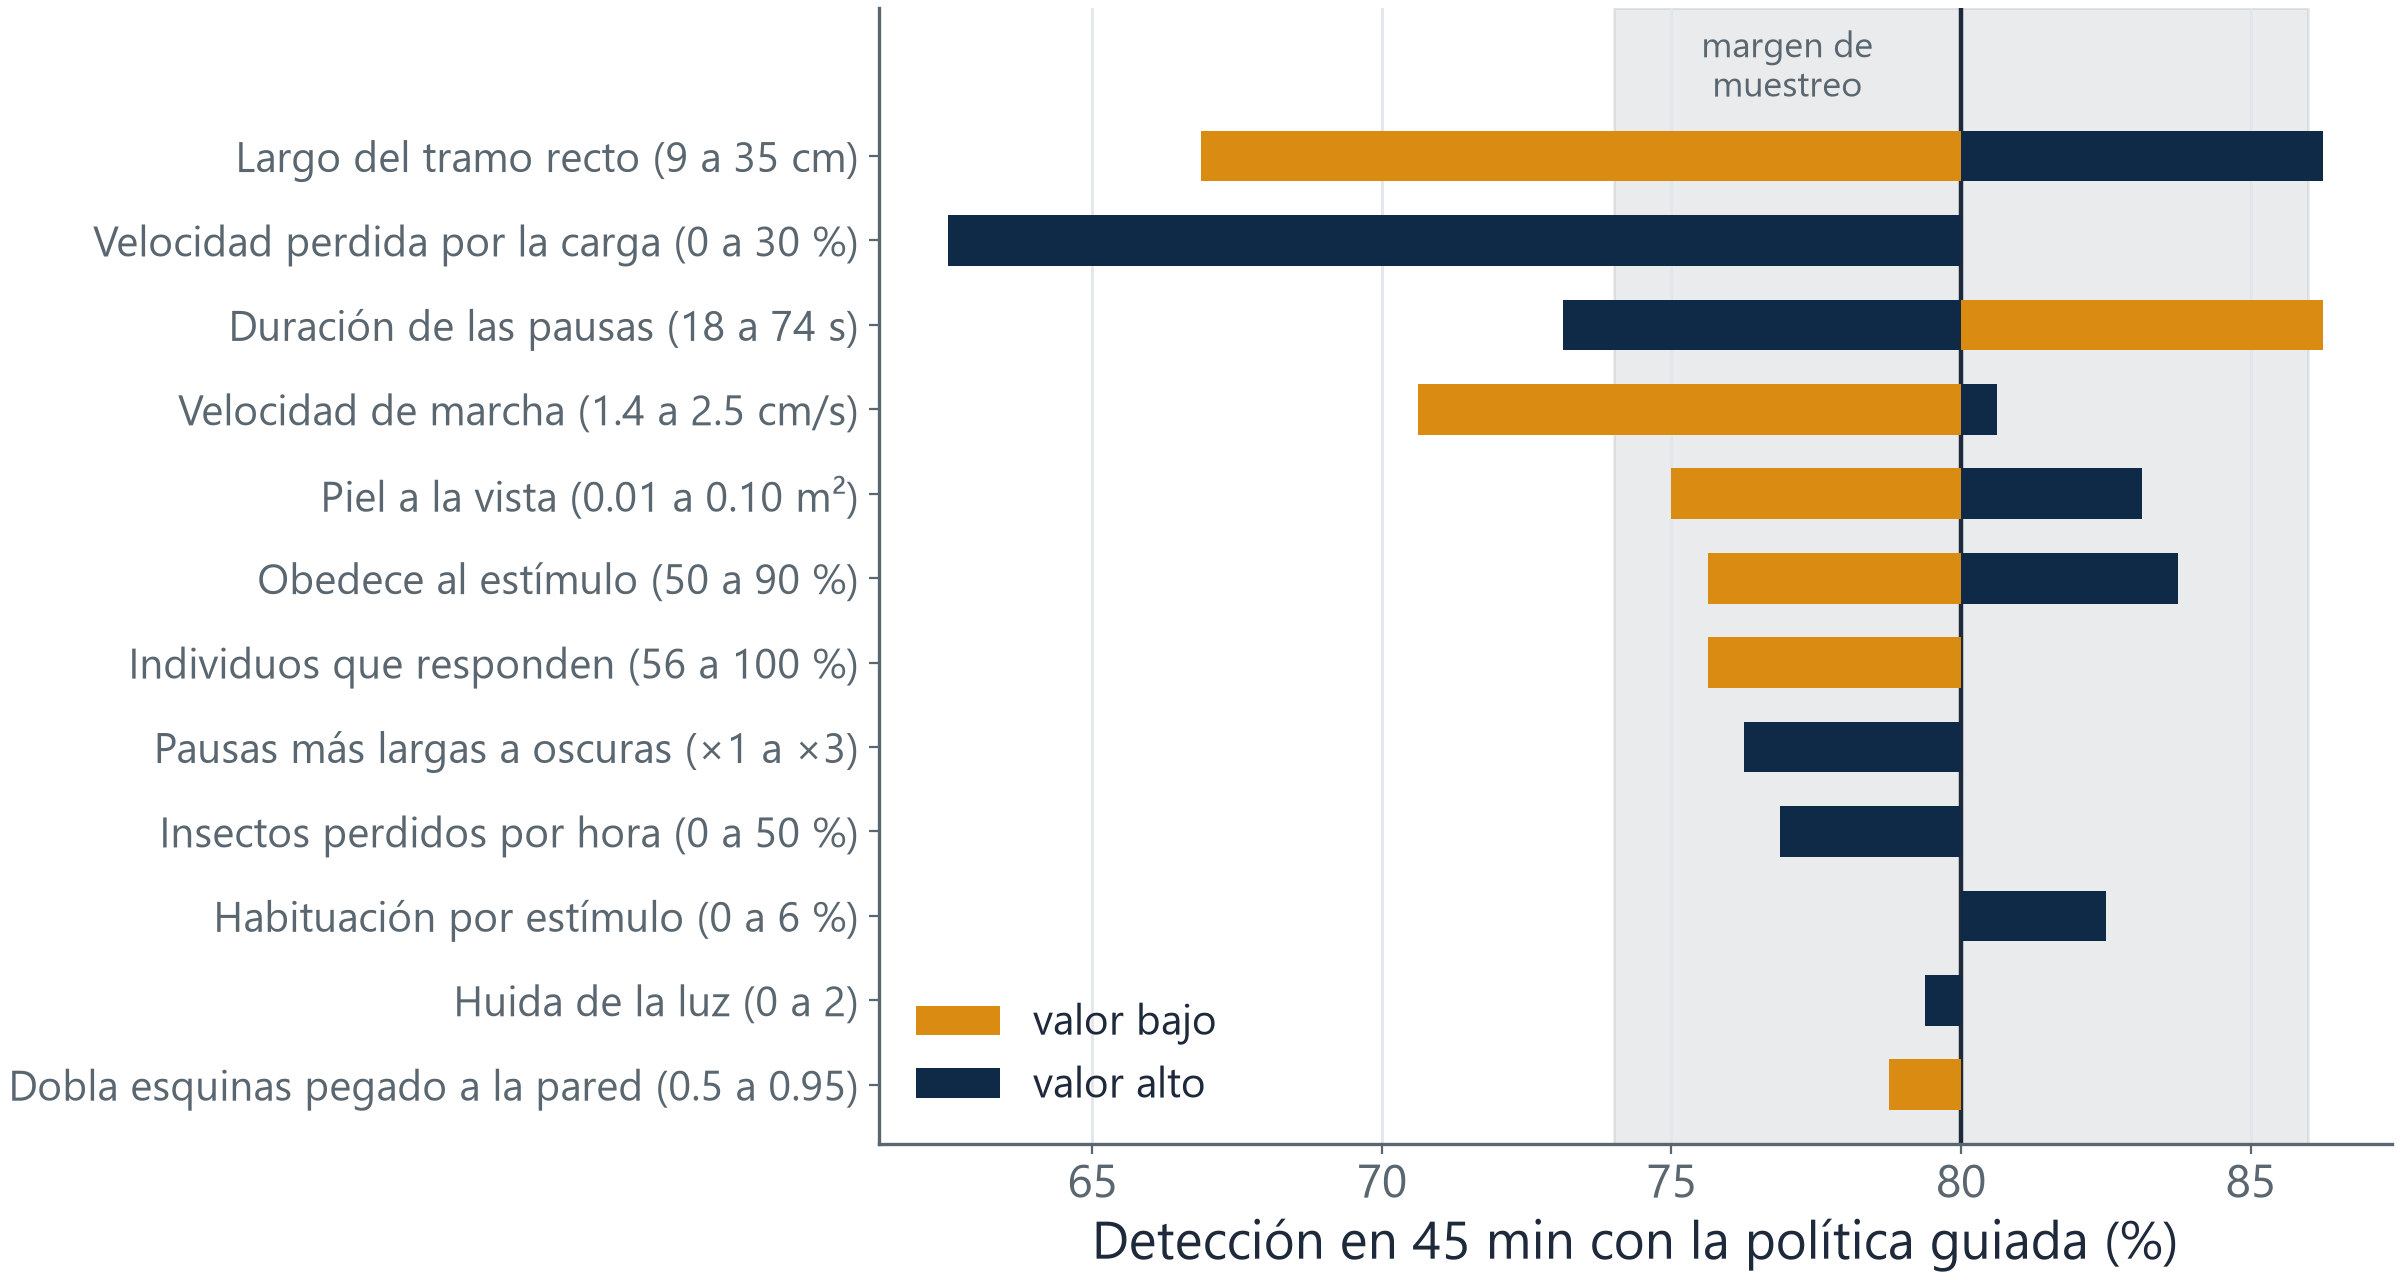
\includegraphics[width=0.78\textwidth]{figs/sensibilidad.png}
\caption{Cambio en la detección a 45~min de la política guiada al mover cada supuesto.}
\label{fig:sensibilidad}
\end{figure}

\textbf{Recuperar a los insectos.}\phantomsection\label{sec:regreso} Tras 45~min de búsqueda se da la orden de
regreso; en el boquete hay un refugio oscuro que retiene a los que pasan a 30~cm (figura~\ref{fig:regreso}
y tabla~\ref{tab:regreso}, \regInsectos{} insectos por caso). Con solo el refugio vuelve \regTrampaSesenta~\% en una hora y \regTrampaDos~\% en
dos. Guiarlo a ciegas es peor: el rumbo recto o desandar la ruta recuperan \regRumboDos{} y \regRutaDos~\%, porque la
cuenta de pasos y giros se desvía con cada metro. Lo que cambia el resultado es una señal en la entrada: con un faro
infrarrojo que se percibe hasta 6~m y dos fotodiodos vuelve \regFaroSesenta~\% en una hora y \regFaroDos~\% en dos,
con \regEstFaro{} estímulos. Ningún método los recupera a todos. El faro es un supuesto: existen sus dos piezas por
separado, una cerca invisible~\cite{latif2014} y la localización de sonido desde la mochila~\cite{latif2016}.

\begin{table}[!htb]
\centering\footnotesize
\caption{Insectos recogidos (\%) después de la orden de regreso y estímulos gastados en volver.}
\label{tab:regreso}
\rowcolors{2}{SoftGray}{white}
\begin{tabularx}{0.9\textwidth}{@{}>{\raggedright\arraybackslash}X r r r r@{}}
\toprule
\rowcolor{TableHead} \textbf{Forma de regresar} & \textbf{30 min} & \textbf{60 min} & \textbf{120 min} & \textbf{Estímulos por insecto} \\
\midrule
\tablaRegreso
\bottomrule
\end{tabularx}
\end{table}

\begin{figure}[!htb]
\centering
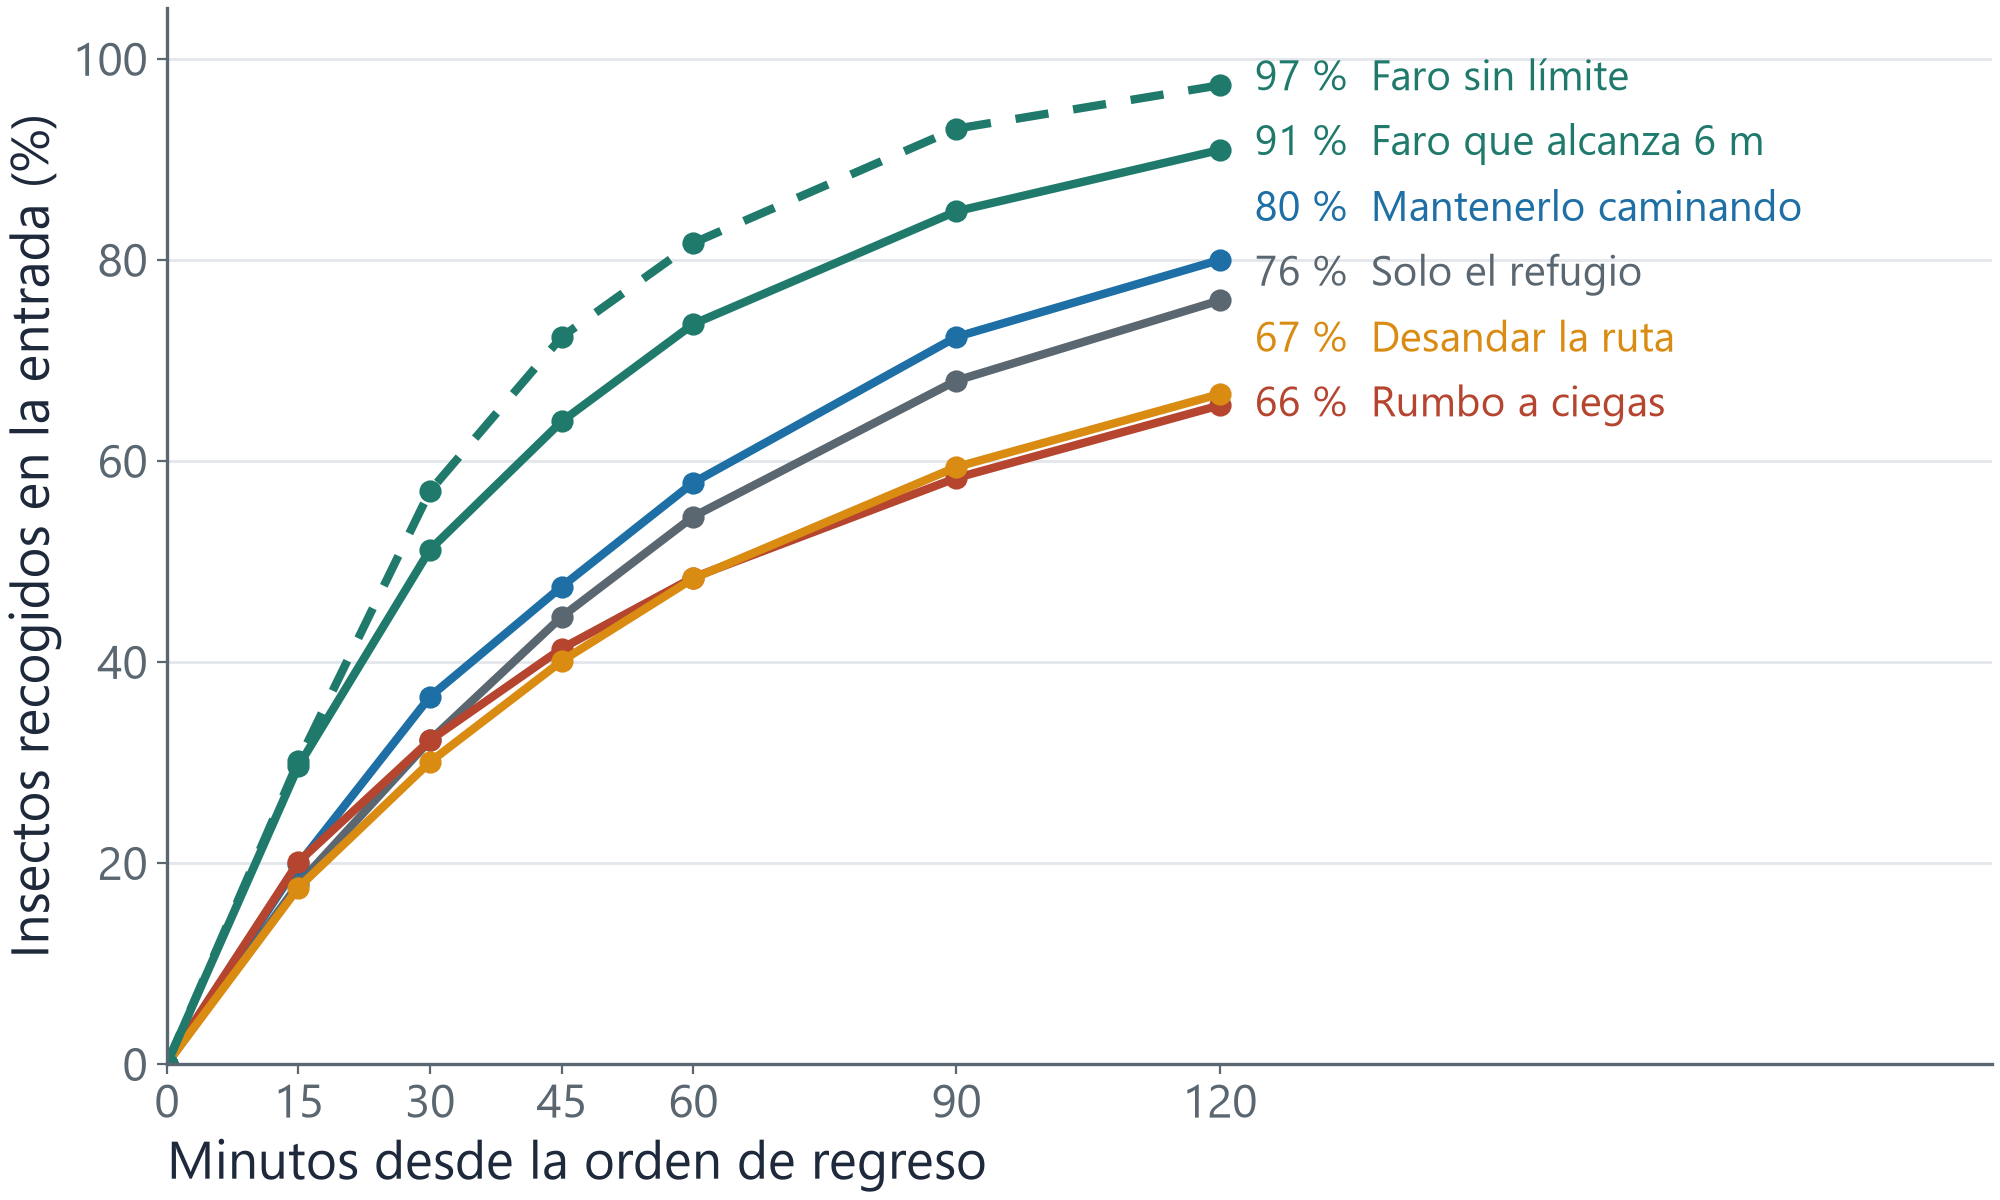
\includegraphics[width=0.70\textwidth]{figs/regreso.png}
\caption{Insectos recogidos en la entrada según la forma de hacerlos volver. La línea punteada es el techo del método.}
\label{fig:regreso}
\end{figure}

\textbf{Qué dice y qué no dice.} La guiada aumenta la detección en 45 a 60~min (de \pPasivaCuarentaCinco{} a
\pGuiadaCuarentaCinco~\% y de \pPasivaSesenta{} a \pGuiadaSesenta~\%) y lo hace con pocos estímulos, pero la mejora
depende del colapso. No dice cuánto tardaría un rescate real, porque los colapsos son planos y la marcha se midió en
arenas iluminadas, ni dice nada sobre falsas alarmas: en la simulación la persona es la única fuente de calor.
